\subsection{Experimental Methods for Colour Constancy Research}

\begin{citequote}{hurlbert_colour_2007}
\emph{How is colour constancy measured?} With difficulty.
\end{citequote}

The following section is divided into two following the split in research methods between those who could be described as coming from a `colour science' perspective (where quantification and specification of colour are primary goals, and the development of \glspl{CAT} is a primary goal) and those coming from a `vision science' perspective (where an understanding of the visual system is the primary goal). Further discussion of this split, and the introduction of a third group, comes in Section \ref{sec:schools}.

\subsubsection{Within Colour Science}

CIE 160:2004 \citep{cie_tc_1-52_cie_2004} and \citet{luo_review_2000} provide a comprehensive overview of the different methods which have been used by the \gls{CAT} group:

\begin{itemize}
\item Haploscopic matching
\item Local Adaptation Matching
\item Memory Matching
\item Magnitude Estimation
\end{itemize}


\paragraph{Haploscopic Matching} is the most common technique in this field, and the term refers to experiments which differentially adapt the two eyes and allow an observer to vary attributes of the stimulus presented to one eye such that it in some way matches the attributes of a fixed stimulus shown to another eye. Whilst this is in many ways unnatural, the benefits are that an experiment can be set up so that there is no time interference (the presentations are simultaneous, so memory effects are avoided) and that high precision of match is relatively easily achieved. An assumption is made that the adaptation of each eye is independent.

\begin{figure}[htbp]
    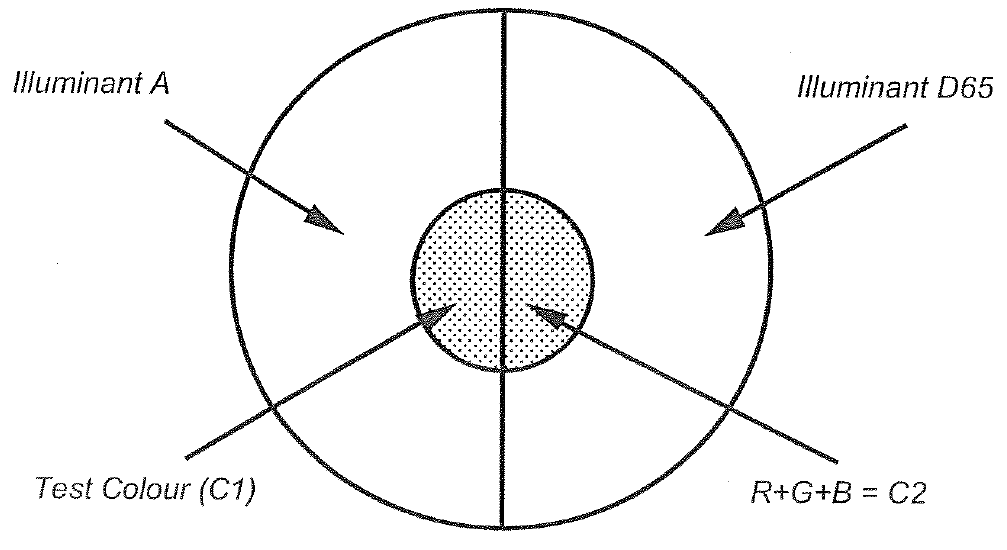
\includegraphics[max width=\textwidth]{figs/LitRev/hapl.png}
    \caption{Figure 11 from \citet{cie_tc_1-52_cie_2004}, showing `A typical viewing condition used in the haploscopic matching experiment'.}
    \label{fig:hapl}
\end{figure} 


\paragraph{Local Adaptation Matching} can be considered as a variation of haploscopic matching where instead of differing adaptational stimuli being presented to each eye, differing adaptational stimuli are presented to different parts of the same eye (spatially distinct areas of the same retina). The assumption here is that there is minimal intra-retinal interaction. MacAdam's 1956 study \citep{macadam_chromatic_1956} epitomises this technique. This experimental technique requires that observers minimise eye movement, in order to maintain spatially distinct adaptation.

\paragraph{Memory Matching} has traditionally been performed by training observers to communicate colour sensation through the Munsell system notation \citep{helson_object-color_1952,lam_metamerism_1985} and then asking observers adapted to different ambient lighting to describe set real objects using such notation. This technique is not much used due to many limitations and confounding factors. \citet{luo_review_2000} details the limitations of this experimental technique succinctly: `a substantial training period being required, complicated procedures for data analysis, lower precision than that of haploscopic technique, limited capacity for retaining information, and memory distortion.'

\paragraph{Magnitude Estimation} appears to be similar to memory matching, in that observers are requested to verbally describe an object whilst in an ambient adapting field. The distinction is that the observers are requested to communicate their perceptions using the perceptually meaningful attributes of hue, saturation and brightness, and as such results can be easily integrated into colour appearance models. Recent experiments \citep{kuo_various_1995,xu_testing_1997,luo_quantifying_1991-1,luo_quantifying_1991,luo_quantifying_1993-1,luo_quantifying_1993} of this type collected data which was used to create CIECAM97s.

\subsubsection{Within Vision Science} \label{sec:methvis} 

Methodologies similar to those described above, but with subtle yet important differences have been used by those whose primary goal is an understanding of the visual system. A valuable overview is provided by \citet{foster_color_2011}, who lists four main methods:

\begin{enumerate}
\item Asymmetric color matching
\item Color naming and related methods
\item Achromatic adjustment
\item Discriminating illumination changes from reflectance changes
\item Illumination discrimination tasks
\end{enumerate}

\paragraph{Asymmetric matching} is in many ways analogous to the haploscopic matching described above, in that it describes an experimental set-up whereby one stimulus is compared with another, generally where each stimulus exists within a distinct adapting field and attributes of one stimulus can be either adjusted or responded to by an observer. The term asymmetric matching might be thought to be inclusive of a wider range of experimental set-ups, where haploscopic (Greek roots: haploieides, single and skopeo, to view) is necessarily concerned with each individual eye receiving distinct input. Asymmetric matching may refer to experiments where stimuli are viewed simultaneously, successively, or in an alternating fashion, binocularly or haploscopically.

\paragraph{Colour Naming} is a technique employed with the aim being a more natural task than  asymmetric matching, and removing some of the `instruction effects' probed by \citet{arend_simultaneous_1986}. \citet{foster_color_2011} argues that colour naming represents a task apt to measure colour constancy more directly, as opposed to the `relational colour constancy' often studied in asymmetric matching experiments, since it concerns identification rather than equivalence. One clear benefit seems to be that the observer needn't be aware of the equivalence; it is expected that in such experiments there will be only one stimulus, perhaps with a temporally variant adapting field. An observer is simply asked to name colours, and this should theoretically result in a measure of adaptational colour constancy as opposed to inferential colour constancy, so long as the stimuli is suitably abstract. Colour names may be of a fixed set, or an observer may be given free choice. Analysis of results can employ a naming centroid based approach or a boundary focused approach. \citet{speigle_is_1996} proposed a novel approach combining magnitude estimation and colour naming with the aim to improve precision of response.

\paragraph{Achromatic Adjustment} experiments ask an observer to set a stimulus to a neutral achromatic hue, on the assumption that the internal grey point of an observer shifts in response to different adapting fields. These adjustments are generally easy for an observer to make, but the extrapolation of the results makes various assumptions about conceptual colour space and the nature of achromacy. Experiments are easily confounded by complex or real stimuli where there exists a close-to-neutral object in the scene which could consciously or unconsciously be used as a reference.

\paragraph{Discriminating illumination changes from reflectance changes} provides a key way to examine colour constancy in an operational manner. Following the assumption that chromatic adaptation allows an observer to discount the illumination in some manner, an experimental set up where observers are requested to distinguish between an illumination change and a reflectance change represents a situation which very closely mirrors the natural process of colour constancy. This experimental technique is well placed to examine whether or not colour constancy in this form is active and efficient, but it provides little way of probing the underlying mechanisms of colour constancy.

\paragraph{Illumination discrimination tasks} comprise a scene which is unvarying in terms of content and surface reflectances, but varying in terms of illumination. In the general set-up (such as that described by \citet{pearce_chromatic_2014}), a target illumination is compared to two test illuminations, where one of the test illuminations is identical to the the target illumination and the other differs in chromaticity. The observer performs a two-alternative forced choice task whereby they attempt to identify the identical illumination, and from this estimates of the observers discrimination thresholds for illuminations of differing chromatic directions away from the test illumination can be estimated. \citet{aston_illumination_2019} describes the interpretation of data from such as experiments as offering two types of insight. Firstly, where no difference can be seen by observers this can be thought of as perfect colour constancy (assuming that the chromaticity differences are above surface discriminability thresholds) and comparisons across different chromatic directions can be made. Secondly, an indication as to the accuracy with which illumination colour is encoded can be gleaned. Concerns regarding this methodology were recently raised by \citet{weiss_determinants_2017} who ``did not find any relationship between achromatic adjustments and illumination discrimination thresholds'' which ``casts doubt on the idea that illumination discrimination directly translates into colour constancy''.

\subsubsection{Achromatic Adjustments under Different Illuminations} \label{sec:aadi}

A number of researchers have performed experiments similar in nature to those reported in Chapters \ref{chap:LargeSphere} and \ref{chap:LargeSphere}, and these are summarised below. These references were added following suggestions by the examining committee for this thesis.

\textbf{\citet{werner_effect_1982}}\footnote{More succinctly reported in \citet{walraven_chromatic_1982}.} performed an achromatic adjustment experiment whereby chromatic annuli (60'-90') were presented as flashed stimuli (3 seconds on, 3 seconds off) on top of a background pedestal of varying chromaticity, and the observer's task was to modify the chromaticity of the annuli such that they appeared achromatic. 

The authors found that the luminance contrast between the background and the annuli had an effect; the higher the contrast between the two, the less saturated the annuli needed to be to appear achromatic. The authors note that ``[t]his is not what should be expected on the basis of a simple von Kries transformation. The latter should yield, for a given background, hue shifts that are the same for dim (low contrast) or bright (high contrast) test stimuli'' \citep{walraven_chromatic_1982}.

The authors also found an effect of the background luminance; higher luminances required more saturated annuli to appear achromatic. 

The authors found that by considering only the chromaticity of the additional annulus (rather than the sum of annulus and background) they could account for the contrast effect (the background luminance effect remaining). Following this type of computation, they could account for the adaptive shifts with receptor-specific gain controls.

\textbf{\citet{brainard_color_1998}} used a method of achromatic adjustment in a slightly more naturalistic condition; a room was built where the ambient lighting could be carefully controlled, and where the chromaticity of a target patch could be controlled by an observer, through use of a projection colorimeter. Munsell papers and `theater stage lamps' were used, and so this set-up was still considerably non-naturalistic compared to a real world environment.

The key findings from this series of experiments were that generally the constancy indices were very high (observers exhibited strong and effective colour constancy), and that the immediate surround of a target patch had very little effect on the achromatic point selected. This second result ``differ[s] from a number of studies in the literature in which local contrast decisively determined appearance''. The reason for this difference was proposed as the greatly increased ``richness of the stimulus conditions.''

The authors also found no discernible effect of the chromaticity of the illumination (in terms of one inducing adaptation to a greater extent than another). This ``contradicts the idea, suggested by a number of theorists, that the visual system could take advantage of the fact that most natural illumination variation is along the daylight locus''.

In contrast to the findings of \citet{werner_effect_1982}, as noted by \citet{aston_what_2017}, \citet{brainard_color_1998} ``found that achromatic settings made at fixed luminance levels lie along a straight line in a three-dimensional cone space, concluding from this that changing [target] luminance did not affect the chromaticity setting of an observer’s achromatic point'' \citep{aston_what_2017}.

\textbf{\citet{kuriki_loci_2006}} starts by referring to the above finding of \citet{brainard_color_1998}, but goes on to note that `many studies have shown that the color appearance of a light of fixed chromaticity varies with its intensity', referring directly to the results of \citet{werner_effect_1982} amongst others, and offering the Helson-Judd effect (whereby `lighter surfaces tend to take on the color of the illuminant') as a concrete example whereby appearance can be seen to change as a direct result of changes in the intensity of surface reflectance.

The author suggests two possible reasons for this discrepancy: the difference between experiments dealing with increments and decrements, and the use of display technologies vs. `real' scenes.

The results from an achromatic setting experiment are described, where a real-world (room-based) environment was used with a screen-based target (though the target is said to have appeared as a piece of paper on the wall). A fitting to the data from this experiment suggests that ``chromatic adaptation is not describable as a change in sensitivity parameters alone for an otherwise linear system. The implied nonlinearity takes the form of an adaptation-dependent change in exponent'', broadly agreeing with the findings of \citet{walraven_chromatic_1982}. The authors note however that the predictions of the model developed by \citet{walraven_chromatic_1982} do not ``agree well with the present data''.

The author also further compares the results to those of \citet{brainard_color_1998}:

\begin{itquote}{}
The results of Brainard’s study on achromatic loci (\citet{brainard_color_1998}) agree with ours in some points, but he found
no pronounced intensity dependence of the entries of the
weighting coefficients for the cone excitations. A possible
cause of the difference is that the present study contained
more higher-lightness conditions than his.
\end{itquote}

\textbf{\citet{weiss_determinants_2017}} report two experiments, one using a colour naming method and one using an achromatic adjustment method, both performed using screen-based stimuli for 40 different chromatic illuminants.

They test a large number of theories of colour constancy (referring to each as a `determinant'), and found limited support for a role of colour naming and a strong blue bias. Additionally, ``[t]here was some evidence that other factors, such as metamer mismatching, relational colour constancy, and colour variegation, play a role in colour constancy, but in a rather complicated way. In any case, the blue bias and the consistency of the illumination categories explained most of the variance of the achromatic adjustments.''





\clearpage

% %recent advances in colour constancy?
% % using more realistic stimuli
% % the grey edges algo
% % the comparison of grey edge and grey world/bright is white

%% Excluded -----------------






% A large range of experimental methods have been used to investigate the problem of colour constancy partly because different experimenters were approaching the problem from different angles aiming to accomplish subtly separate goals.

% Those interested in developing \glspl{CAT}, focusing on chromatic adaptation

% Those approaching from a mathematical perspective (perhaps with the mind-set `if we find the algorithm which predicts corresponding colours a) this is very useful for industry and b) we can then work backwards to explain how human colour constancy may occur') are concerned primarily with producing chromatic adaptation transforms.

% Those approaching colour constancy with a basic interest in the physiology and general function of colour constancy have adopted/created a rather wider set of experimental techniques, owing to the fact that this direction of study is much less well broader than the former

